% =============================================================================
%  Diplomado en Data Science Aplicada con Python para la Toma de Decisiones
%  Clase 14: De Regresión a Clasificación — Regresión Logística
%  Arca Continental Ecuador | UDLA
%
%  Compilar: pdflatex -shell-escape presentacion.tex (x2 para refs)
% =============================================================================
\documentclass[aspectratio=169, 11pt]{beamer}

\usepackage[T1]{fontenc}
\usepackage[utf8]{inputenc}
\usepackage[spanish,es-noshorthands]{babel}
\usepackage{FiraSans}
\usepackage{FiraMono}
\renewcommand{\familydefault}{\sfdefault}
\usepackage{graphicx}
\usepackage{tikz}
\usetikzlibrary{arrows.meta, positioning, shapes.geometric, shapes.misc,
  calc, fit, decorations.pathreplacing, backgrounds}
\usepackage{fontawesome5}
\usepackage{minted}
\usepackage{tcolorbox}
\tcbuselibrary{minted, skins, breakable}
\usepackage{booktabs}
\usepackage{colortbl}
\usepackage{multicol}
\usepackage{hyperref}
\usepackage{calc}
\usepackage{amsmath}

\definecolor{arcaRed}{HTML}{C82B40}
\definecolor{arcaDark}{HTML}{6B1525}
\definecolor{udlaCrimson}{HTML}{A31545}
\definecolor{arcaGray}{HTML}{F5F5F5}
\definecolor{arcaLightGray}{HTML}{EBEBEB}
\definecolor{textDark}{HTML}{2D2D2D}
\definecolor{textMuted}{HTML}{6B7280}
\definecolor{codeGreen}{HTML}{16A34A}
\definecolor{codeBlue}{HTML}{2563EB}
\definecolor{codeOrange}{HTML}{EA580C}
\definecolor{codePurple}{HTML}{7C3AED}

\usetheme{default}
\usecolortheme{default}
\setbeamertemplate{navigation symbols}{}
\setbeamertemplate{footline}{}
\setbeamertemplate{headline}{}
\setbeamercolor{normal text}{fg=textDark}
\setbeamercolor{frametitle}{fg=arcaRed, bg=white}
\setbeamercolor{title}{fg=white}
\setbeamercolor{subtitle}{fg=white!85}
\setbeamercolor{author}{fg=white!80}
\setbeamercolor{date}{fg=white!70}
\setbeamercolor{item}{fg=arcaRed}
\setbeamercolor{subitem}{fg=arcaDark}
\setbeamercolor{block title}{fg=white, bg=arcaRed}
\setbeamercolor{block body}{fg=textDark, bg=arcaGray}
\setbeamercolor{block title alerted}{fg=white, bg=codeOrange}
\setbeamercolor{block body alerted}{fg=textDark, bg=arcaGray}
\setbeamercolor{block title example}{fg=white, bg=codeGreen}
\setbeamercolor{block body example}{fg=textDark, bg=arcaGray}
\setbeamercolor{section in toc}{fg=arcaDark}
\setbeamerfont{frametitle}{size=\Large, series=\bfseries}
\setbeamerfont{title}{size=\huge, series=\bfseries}
\setbeamerfont{subtitle}{size=\large}
\setbeamerfont{author}{size=\normalsize}
\setbeamerfont{date}{size=\small}
\setbeamerfont{block title}{size=\normalsize, series=\bfseries}
\setbeamerfont{footnote}{size=\tiny}
\setbeamertemplate{itemize item}{\scriptsize\raise1.5pt\hbox{\color{arcaRed}$\blacktriangleright$}}
\setbeamertemplate{itemize subitem}{\scriptsize\raise1pt\hbox{\color{arcaDark}$\bullet$}}
\setbeamertemplate{enumerate items}[default]
\setbeamercolor{enumerate item}{fg=arcaRed}

\setbeamertemplate{headline}{%
  \begin{tikzpicture}[remember picture, overlay]
    \fill[arcaDark] (current page.north west) rectangle
      ([yshift=-0.7cm]current page.north east);
    \node[anchor=west, inner sep=0pt] at
      ([xshift=0.6cm, yshift=-0.35cm]current page.north west)
      {
\includegraphics[height=0.45cm]{../logo_udla_white.png}};
    \node[anchor=east, inner sep=0pt] at
      ([xshift=-0.6cm, yshift=-0.35cm]current page.north east)
      {
\includegraphics[height=0.45cm]{../ArcaContinental_white.png}};
  \end{tikzpicture}%
  \vspace{0.7cm}%
}

\setbeamertemplate{footline}{%
  \begin{tikzpicture}[remember picture, overlay]
    \node[anchor=south east, font=\scriptsize\bfseries\color{arcaRed}] at
      ([xshift=-0.5cm, yshift=0.15cm]current page.south east)
      {\insertframenumber};
  \end{tikzpicture}%
  \vspace{0.3cm}%
}

\setbeamertemplate{frametitle}{%
  \vspace{0.25cm}%
  \usebeamerfont{frametitle}\usebeamercolor[fg]{frametitle}\insertframetitle%
  \par\vspace{2pt}%
  \begin{tikzpicture}
    \fill[arcaRed] (0,0) rectangle (3cm, 1.5pt);
    \fill[arcaLightGray] (3cm,0) rectangle (\textwidth, 0.5pt);
  \end{tikzpicture}%
  \vspace{0.1cm}%
}

\newtcblisting{pyblock}[1][]{%
  listing engine=minted, minted language=python, minted style=friendly,
  minted options={fontsize=\small, linenos=false, breaklines=true, python3=true},
  colback=arcaGray, colframe=arcaRed, left=4pt, right=4pt, top=4pt, bottom=4pt,
  boxrule=0pt, leftrule=3pt, arc=2pt, listing only, #1}

\newtcblisting{outputblock}[1][]{%
  listing engine=minted, minted language=text, minted style=bw,
  minted options={fontsize=\small, breaklines=true},
  colback=white, colframe=arcaLightGray, left=4pt, right=4pt, top=4pt, bottom=4pt,
  boxrule=0.5pt, arc=2pt, listing only,
  title={\small\faTerminal\hspace{6pt}Output}, coltitle=textMuted,
  fonttitle=\small\ttfamily, colbacktitle=white, #1}

\newcommand{\sectionframe}[2]{%
  \begingroup
  \setbeamertemplate{headline}{}%
  \setbeamertemplate{footline}{}%
  \begin{frame}[plain, noframenumbering]
    \begin{tikzpicture}[remember picture, overlay]
      \fill[arcaRed] (current page.south west) rectangle (current page.north east);
      \node[anchor=center, text=white, font=\Huge\bfseries, text width=12cm,
            align=center] at ([yshift=0.5cm]current page.center) {#1};
      \node[anchor=center, text=white!80, font=\large, text width=10cm,
            align=center] at ([yshift=-0.8cm]current page.center) {#2};
    \end{tikzpicture}
  \end{frame}
  \endgroup
}

\title{Diplomado en Data Science Aplicada\\con Python para la Toma de Decisiones}
\subtitle{Clase 14: De Regresión a Clasificación}
\author{Carlos Enrique Mosquera Trujillo}
\date{10 de Abril, 2026}

\begin{document}

% ── PORTADA ──────────────────────────────────────────────────────────────────
{
\setbeamertemplate{headline}{}
\setbeamertemplate{footline}{}
\begin{frame}[plain, noframenumbering]
  \begin{tikzpicture}[remember picture, overlay]
    \fill[arcaDark] (current page.south west) rectangle (current page.north east);
    \fill[arcaRed] ([yshift=-3.5cm]current page.north west) rectangle
      ([yshift=-4.2cm]current page.north east);
    \node[anchor=west, inner sep=0pt] at
      ([xshift=1cm, yshift=-1.5cm]current page.north west)
      {
\includegraphics[height=1cm]{../logo_udla_white.png}};
    \node[anchor=east, inner sep=0pt] at
      ([xshift=-1cm, yshift=-1.5cm]current page.north east)
      {
\includegraphics[height=1cm]{../ArcaContinental_white.png}};
  \end{tikzpicture}
  \vspace{2.5cm}
  \begin{center}
    {\usebeamerfont{title}\usebeamercolor[fg]{title}\inserttitle\par}
    \vspace{0.4cm}
    {\usebeamerfont{subtitle}\usebeamercolor[fg]{subtitle}\insertsubtitle\par}
    \vspace{0.6cm}
    {\usebeamerfont{author}\usebeamercolor[fg]{author}\insertauthor\par}
    \vspace{0.15cm}
    {\usebeamerfont{date}\usebeamercolor[fg]{date}\insertdate\par}
  \end{center}
\end{frame}
}

% ── MÓDULO 2 ─────────────────────────────────────────────────────────────────
{
\setbeamertemplate{headline}{}
\setbeamertemplate{footline}{}
\begin{frame}[plain, noframenumbering]
  \begin{tikzpicture}[remember picture, overlay]
    \fill[arcaDark] (current page.south west) rectangle (current page.north east);
    \node[anchor=center, text=white, font=\Large\bfseries, text width=12cm,
          align=center] at ([yshift=1cm]current page.center)
      {Módulo 2 --- última clase};
    \node[anchor=center, text=white!90, font=\huge\bfseries, text width=12cm,
          align=center] at ([yshift=-0.3cm]current page.center)
      {Estadística Aplicada para Datos};
  \end{tikzpicture}
\end{frame}
}

% ── RECAPITULACIÓN ──────────────────────────────────────────────────────────
\begin{frame}[shrink=5]{Recapitulación: Clase 13}
  \vspace{-4pt}
  \begin{columns}[T]
    \begin{column}{0.48\textwidth}
      {\footnotesize\bfseries\color{arcaDark} Lo que aprendimos:}
      \vspace{4pt}

      {\footnotesize
      \begin{itemize}\setlength{\itemsep}{4pt}
        \item[{\color{codeGreen}\faCheckCircle}]
          Regresión lineal: simple y múltiple.
        \item[{\color{codeGreen}\faCheckCircle}]
          Interpretar coeficientes en negocio.
        \item[{\color{codeGreen}\faCheckCircle}]
          MSE, RMSE, MAE, R\textsuperscript{2}.
        \item[{\color{codeGreen}\faCheckCircle}]
          Estandarización y train/test split.
      \end{itemize}
      }
    \end{column}

    \begin{column}{0.48\textwidth}
      {\footnotesize\bfseries\color{arcaRed} Hoy completamos el módulo:}
      \vspace{4pt}

      {\footnotesize
      \begin{itemize}\setlength{\itemsep}{4pt}
        \item[{\color{arcaRed}\faArrowRight}]
          P-values: ¿el coeficiente es real o ruido?
        \item[{\color{arcaRed}\faArrowRight}]
          Selección de variables.
        \item[{\color{arcaRed}\faArrowRight}]
          Cuándo NO funciona la regresión lineal.
        \item[{\color{arcaRed}\faArrowRight}]
          Tu primer clasificador: regresión logística.
      \end{itemize}
      }
    \end{column}
  \end{columns}
\end{frame}

% ── ROADMAP ─────────────────────────────────────────────────────────────────
\begin{frame}[shrink=22]{Hoja de Ruta de Hoy}
  \vspace{-4pt}
  \begin{center}
  \begin{tikzpicture}[
    node distance=0.32cm,
    roadstep/.style={rectangle, rounded corners=4pt, draw=arcaRed, fill=arcaRed!8,
                 minimum width=11cm, minimum height=0.6cm,
                 font=\footnotesize\bfseries\color{arcaDark}, align=left,
                 text width=10cm, inner sep=6pt},
    num/.style={circle, fill=arcaRed, text=white, font=\scriptsize\bfseries,
                minimum size=0.5cm, inner sep=0pt},
  ]
    \node[roadstep] (s1) {\hspace{0.8cm}P-values --- ¿este coeficiente es real?};
    \node[roadstep, below=of s1] (s2) {\hspace{0.8cm}Selección de variables --- ¿cuáles quito?};
    \node[roadstep, below=of s2] (s3) {\hspace{0.8cm}Supuestos --- cuándo NO funciona la regresión lineal};
    \node[roadstep, below=of s3] (s4) {\hspace{0.8cm}El problema --- ¿y si el target es sí/no?};
    \node[roadstep, below=of s4] (s5) {\hspace{0.8cm}Regresión lineal para clasificar --- funciona, pero\ldots};
    \node[roadstep, below=of s5] (s6) {\hspace{0.8cm}Regresión logística --- la sigmoide y predict\_proba};
    \node[roadstep, below=of s6] (s7) {\hspace{0.8cm}Cierre del Módulo 2};

    \node[num] at ([xshift=0.45cm]s1.west) {1};
    \node[num] at ([xshift=0.45cm]s2.west) {2};
    \node[num] at ([xshift=0.45cm]s3.west) {3};
    \node[num] at ([xshift=0.45cm]s4.west) {4};
    \node[num] at ([xshift=0.45cm]s5.west) {5};
    \node[num] at ([xshift=0.45cm]s6.west) {6};
    \node[num] at ([xshift=0.45cm]s7.west) {7};
  \end{tikzpicture}
  \end{center}
\end{frame}

% =============================================================================
%  BLOQUE A: CIERRE DE REGRESIÓN LINEAL
% =============================================================================
\sectionframe{Cierre de Regresión Lineal}{Supuestos, p-values y selección de variables}

% ── SUPUESTOS ───────────────────────────────────────────────────────────────
\begin{frame}[shrink=8]{¿Qué Asume la Regresión Lineal?}
  \vspace{-4pt}
  {\footnotesize\color{arcaDark}\bfseries
    Cuando usamos \texttt{LinearRegression}, el modelo \textbf{asume}
    ciertas cosas sobre los datos. Si no se cumplen, los resultados
    pueden ser incorrectos.}

  \vspace{6pt}
  {\scriptsize
  \begin{tabular}{@{}lp{5.2cm}p{4.5cm}@{}}
    \toprule
    \textbf{Supuesto} & \textbf{Qué asume} & \textbf{Si se viola\ldots} \\
    \midrule
    \textbf{Linealidad} &
      La relación entre $X$ e $y$ es una \textbf{línea recta}
      (no una curva ni una escalera). &
      La recta no va a capturar la forma real $\to$
      predicciones sesgadas. \\[3pt]
    \textbf{Independencia} &
      Cada observación es \textbf{independiente} de las demás
      (fila 5 no depende de fila 4). &
      Los errores estándar son incorrectos
      $\to$ p-values no confiables. \\[3pt]
    \textbf{Homocedasticidad} &
      La \textbf{varianza del error} es constante
      (el modelo no se equivoca más en unas zonas que en otras). &
      Las predicciones son ``más dudosas'' en ciertas zonas. \\[3pt]
    \textbf{Normalidad} &
      Los \textbf{residuos} siguen una distribución
      \textbf{aproximadamente Normal}. &
      Los intervalos de confianza y p-values pierden validez. \\[3pt]
    \textbf{No multicolinealidad} &
      Las features no están \textbf{muy correlacionadas} entre sí. &
      Los coeficientes se vuelven inestables
      (cambian mucho si quitas una variable). \\
    \bottomrule
  \end{tabular}
  }
\end{frame}

\begin{frame}{Cómo Verificar: Mirar los Residuos}
  \vspace{-4pt}
  {\footnotesize\color{arcaDark}\bfseries
    La forma práctica de verificar varios supuestos a la vez: graficar
    los residuos vs la predicción.}

  \vspace{4pt}
  \begin{center}
    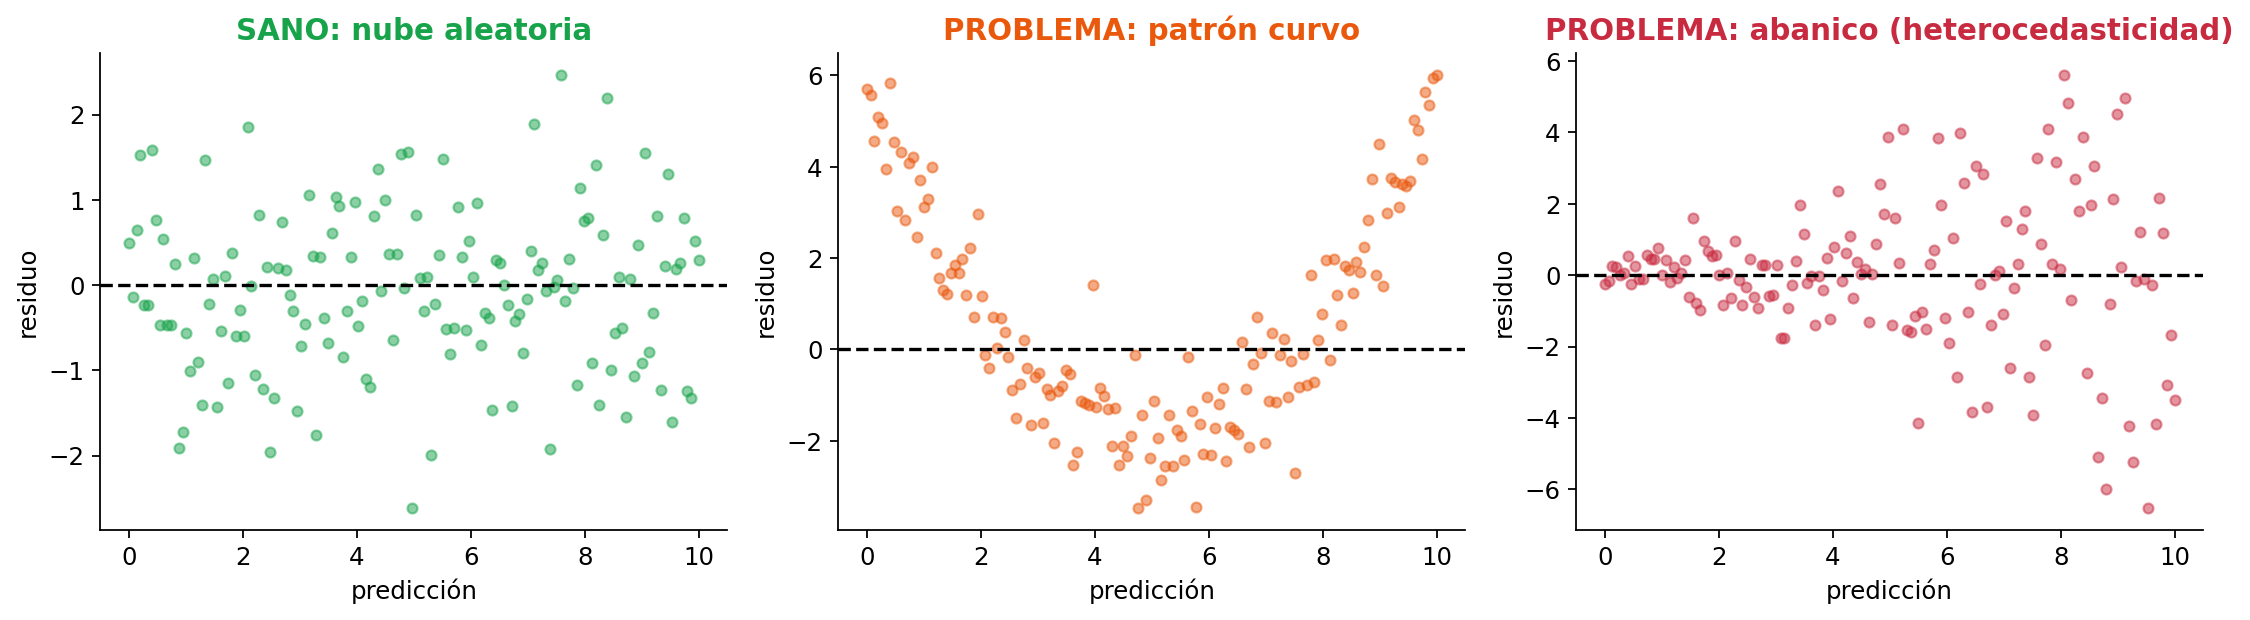
\includegraphics[width=0.92\textwidth]{img_supuestos_residuos.png}
  \end{center}

  \vspace{-2pt}
  {\scriptsize\color{textMuted}
  \begin{itemize}\setlength{\itemsep}{2pt}
    \item[{\color{codeGreen}\scriptsize\faCheckCircle}]
      \textbf{Sano}: nube aleatoria $\to$ linealidad y homocedasticidad OK.
    \item[{\color{codeOrange}\scriptsize\faExclamationTriangle}]
      \textbf{Curvo}: se viola linealidad $\to$ necesitas un modelo no lineal.
    \item[{\color{arcaRed}\scriptsize\faTimesCircle}]
      \textbf{Abanico}: se viola homocedasticidad $\to$ errores desiguales.
  \end{itemize}
  }
\end{frame}

% ── STATSMODELS ─────────────────────────────────────────────────────────────
\begin{frame}[shrink=5]{Nueva Librería: \texttt{statsmodels}}
  \vspace{-4pt}
  {\footnotesize\color{arcaDark}\bfseries
    \texttt{sklearn} entrena modelos pero no calcula p-values.
    Para eso existe \texttt{statsmodels}: una librería enfocada
    en el \textbf{análisis estadístico} de los modelos.}

  \vspace{6pt}
  \begin{columns}[T]
    \begin{column}{0.48\textwidth}
      {\footnotesize\bfseries\color{codeBlue}\faCogs\hspace{4pt}
        sklearn:}
      \vspace{4pt}

      {\scriptsize
      \begin{itemize}\setlength{\itemsep}{4pt}
        \item Orientado a \textbf{predecir}.
        \item API: \texttt{fit / predict / score}.
        \item No reporta p-values ni errores estándar.
        \item Ideal para producción.
      \end{itemize}
      }
    \end{column}

    \begin{column}{0.48\textwidth}
      {\footnotesize\bfseries\color{codePurple}\faChartBar\hspace{4pt}
        statsmodels:}
      \vspace{4pt}

      {\scriptsize
      \begin{itemize}\setlength{\itemsep}{4pt}
        \item Orientado a \textbf{entender}.
        \item API: \texttt{OLS(y, X).fit()}.
        \item Reporta coeficientes, errores estándar,
          \textbf{p-values}, intervalos de confianza.
        \item Ideal para análisis y reportes.
      \end{itemize}
      }
    \end{column}
  \end{columns}

  \vspace{6pt}
  {\footnotesize\color{arcaDark}
    \faLightbulb\hspace{4pt}
    Ambas calculan \textbf{la misma regresión} (mínimos cuadrados).
    Solo difieren en lo que \textbf{reportan}.}
\end{frame}

\begin{frame}[fragile,shrink=35]{Calcular P-values con \texttt{statsmodels}}
  \vspace{-6pt}
  {\footnotesize\color{arcaDark}\bfseries
    Ajustamos el mismo modelo de insurance, ahora con \texttt{statsmodels}.}

  \vspace{4pt}
  \begin{pyblock}
import statsmodels.api as sm

# add_constant agrega la columna del intercepto
# (sklearn lo hace solo, statsmodels no)
X_sm = sm.add_constant(X_train)

# OLS = Ordinary Least Squares (minimos cuadrados)
modelo_sm = sm.OLS(y_train, X_sm).fit()

# .pvalues tiene el p-value de cada coeficiente
print(modelo_sm.pvalues.round(4))
  \end{pyblock}
\end{frame}

% ── P-VALUES ────────────────────────────────────────────────────────────────
\begin{frame}[shrink=5]{¿Qué Pregunta el P-value?}
  \vspace{-4pt}
  {\footnotesize\color{arcaDark}\bfseries
    Cada coeficiente $\beta$ es una \textbf{estimación} a partir de una
    muestra. El p-value mide qué tan confiable es esa estimación.}

  \vspace{6pt}
  {\footnotesize
  \begin{itemize}\setlength{\itemsep}{6pt}
    \item[{\color{arcaRed}\faArrowRight}]
      El modelo dice $\beta_{\text{sex}} = -131$.
      Pero si tomamos \textbf{otra muestra} de 1338 personas,
      podría salir $+50$ o $-300$.
    \item[{\color{arcaRed}\faArrowRight}]
      El p-value pregunta: \textit{``¿podría ser que el verdadero
      $\beta$ sea \textbf{cero} y lo que veo sea solo ruido?''}
    \item[{\color{arcaRed}\faArrowRight}]
      Si \textbf{p $<$ 0.05}: es muy improbable que sea cero
      $\to$ confío en que esta variable \textbf{sí aporta}.
    \item[{\color{arcaRed}\faArrowRight}]
      Si \textbf{p $>$ 0.05}: no puedo descartar que sea cero
      $\to$ esta variable \textbf{quizás no aporta nada}.
  \end{itemize}
  }
\end{frame}

\begin{frame}[shrink=20]{La Matemática del P-value: de $\hat{\beta}$ a $t$ a $p$}
  \vspace{-4pt}
  {\footnotesize\color{arcaDark}\bfseries
    Tres pasos. El último lo hace \texttt{statsmodels} por nosotros.}

  \vspace{8pt}
  {\footnotesize
  \textbf{1.\ El error estándar SE($\hat{\beta}$)}: mide cuánto variaría
  el coeficiente si tuviéramos otra muestra. Se calcula a partir de
  los residuos y la dispersión de las features (más datos o más
  dispersión $\to$ SE más bajo $\to$ más certeza).

  \vspace{6pt}
  \textbf{2.\ El estadístico $t$}: el coeficiente dividido entre su incertidumbre.
  }

  \vspace{4pt}
  \begin{center}
    \begin{tcolorbox}[colback=arcaGray, colframe=arcaRed, boxrule=1pt,
                      arc=4pt, width=0.45\textwidth]
    \centering
    \large
    $t = \dfrac{\hat{\beta}}{\text{SE}(\hat{\beta})}$
    \end{tcolorbox}
  \end{center}

  \vspace{4pt}
  {\footnotesize
  Ejemplo: \texttt{age} $\to$ $t = 257/13.2 = 19.4$ (lejos de cero).
  \texttt{sex\_male} $\to$ $t = -19/372 = -0.05$ (prácticamente cero).

  \vspace{6pt}
  \textbf{3.\ El p-value}: se obtiene de la \textbf{distribución $t$ de Student}
  (una campana similar a la Normal, pero con colas más anchas cuando
  hay pocos datos). El p-value es el área en las colas: si $|t|$ es
  grande, el área es chica $\to$ p-value bajo $\to$ significativo.
  }
\end{frame}

\begin{frame}{Paso 2: de $t$ al P-value}
  \vspace{-4pt}
  {\footnotesize\color{arcaDark}\bfseries
    Tenemos $t$. El p-value es el \textbf{área en las colas} de la
    distribución $t$ de Student.}

  \vspace{4pt}
  \begin{center}
    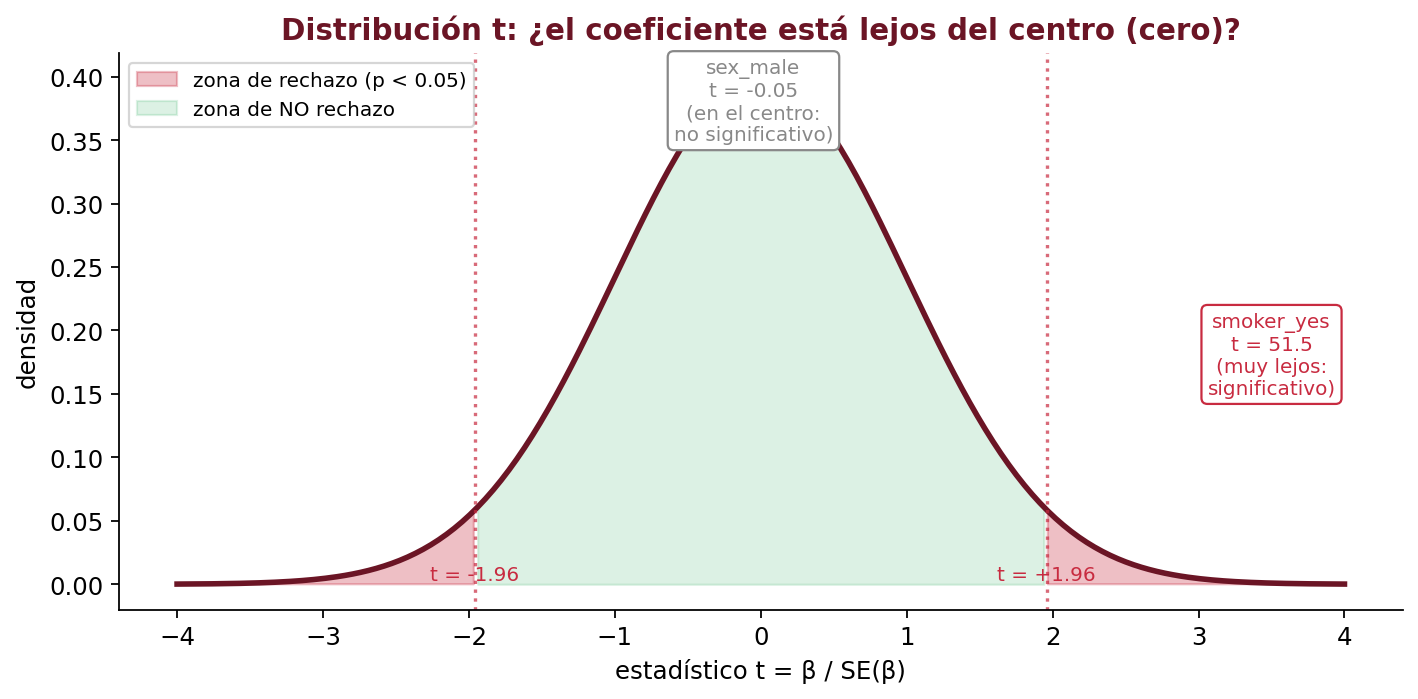
\includegraphics[width=0.68\textwidth]{img_t_statistic.png}
  \end{center}

  \vspace{-2pt}
  {\scriptsize\color{textMuted}
  \begin{itemize}\setlength{\itemsep}{3pt}
    \item[{\color{arcaRed}\scriptsize\faArrowRight}]
      Si $|t|$ es \textbf{grande} (cae en las colas rojas) $\to$
      área chica $\to$ \textbf{p-value bajo} $\to$ significativo.
    \item[{\color{arcaRed}\scriptsize\faArrowRight}]
      Si $|t|$ es \textbf{pequeño} (queda en el centro verde) $\to$
      área grande $\to$ \textbf{p-value alto} $\to$ no significativo.
    \item[{\color{arcaRed}\scriptsize\faArrowRight}]
      \textbf{p-value} $=$ la probabilidad de ver un $t$ tan extremo
      \textbf{si el coeficiente real fuera cero}. Si es $<$ 0.05,
      descartamos que sea cero.
  \end{itemize}
  }
\end{frame}

\begin{frame}[shrink=8]{P-values de Nuestro Modelo de Insurance}
  \vspace{-4pt}
  {\footnotesize\color{arcaDark}\bfseries
    Tabla completa con coeficientes, estadístico $t$ y p-values.}

  \vspace{6pt}
  {\scriptsize
  \begin{tabular}{@{}lrrrl@{}}
    \toprule
    \textbf{Variable} & \textbf{$\hat{\beta}$} & \textbf{$t$} &
      \textbf{p-value} & \textbf{¿Significativa?} \\
    \midrule
    smoker\_yes & $+23\,651$ & 51.5 & 0.000 &
      {\color{codeGreen}\faCheckCircle\hspace{2pt} Sí} \\
    age & $+257$ & 19.4 & 0.000 &
      {\color{codeGreen}\faCheckCircle\hspace{2pt} Sí} \\
    bmi & $+337$ & 10.4 & 0.000 &
      {\color{codeGreen}\faCheckCircle\hspace{2pt} Sí} \\
    children & $+425$ & 2.7 & 0.007 &
      {\color{codeGreen}\faCheckCircle\hspace{2pt} Sí} \\
    region\_southeast & $-658$ & $-1.2$ & 0.218 &
      {\color{codeOrange}\faExclamationTriangle\hspace{2pt} No claro} \\
    region\_southwest & $-810$ & $-1.5$ & 0.123 &
      {\color{codeOrange}\faExclamationTriangle\hspace{2pt} No claro} \\
    region\_northwest & $-371$ & $-0.7$ & 0.484 &
      {\color{arcaRed}\faTimesCircle\hspace{2pt} Ruido} \\
    sex\_male & $-19$ & $-0.05$ & 0.960 &
      {\color{arcaRed}\faTimesCircle\hspace{2pt} Ruido} \\
    \bottomrule
  \end{tabular}
  }

  \vspace{6pt}
  {\footnotesize\color{arcaDark}
    \faLightbulb\hspace{4pt}
    \texttt{sex\_male}: $t = -0.05$, p = 0.96. Los \$19 de diferencia
    son \textbf{indistinguibles de cero}. El sexo no aporta nada.}
\end{frame}

% ── SELECCIÓN DE VARIABLES ──────────────────────────────────────────────────
\begin{frame}[shrink=5]{Selección de Variables: ¿Cuáles Quito?}
  \vspace{-4pt}
  {\footnotesize\color{arcaDark}\bfseries
    Tres criterios prácticos para decidir si una variable se queda o se va.}

  \vspace{6pt}
  {\scriptsize
  \begin{tabular}{@{}lp{5cm}p{4.5cm}@{}}
    \toprule
    \textbf{Criterio} & \textbf{Cómo funciona} & \textbf{Cuándo usarlo} \\
    \midrule
    \textbf{P-value} &
      Si p $>$ 0.05, el coeficiente puede ser cero $\to$ candidata a quitar. &
      Para entender \textbf{qué variables son significativas}. \\[4pt]
    \textbf{Coef.\ estandarizado} &
      Si el coeficiente estandarizado es $\approx$ 0 comparado con los demás $\to$
      poca importancia. &
      Para hacer un \textbf{ranking de importancia}. \\[4pt]
    \textbf{Comparar en test} &
      Entrena CON y SIN la variable. Si MAE/RMSE en test no cambia $\to$
      quítala. &
      \textbf{El más práctico}: mide el impacto real. \\
    \bottomrule
  \end{tabular}
  }

  \vspace{6pt}
  {\footnotesize\color{arcaDark}
    \faLightbulb\hspace{4pt}
    \textbf{Los tres suelen coincidir}: \texttt{sex} y \texttt{region} tienen
    p-values altos, coeficientes estandarizados bajos, y quitarlas no cambia
    el MAE.}
\end{frame}

% ── FLUJO SKLEARN ───────────────────────────────────────────────────────────
\begin{frame}{El Patrón de \texttt{sklearn}: Crear $\to$ Fit $\to$ Predict}
  \vspace{-4pt}
  {\footnotesize\color{arcaDark}\bfseries
    Antes de pasar a un nuevo modelo, fijemos el patrón que
    \texttt{sklearn} usa para \textbf{todos} sus modelos.}

  \vspace{4pt}
  \begin{center}
    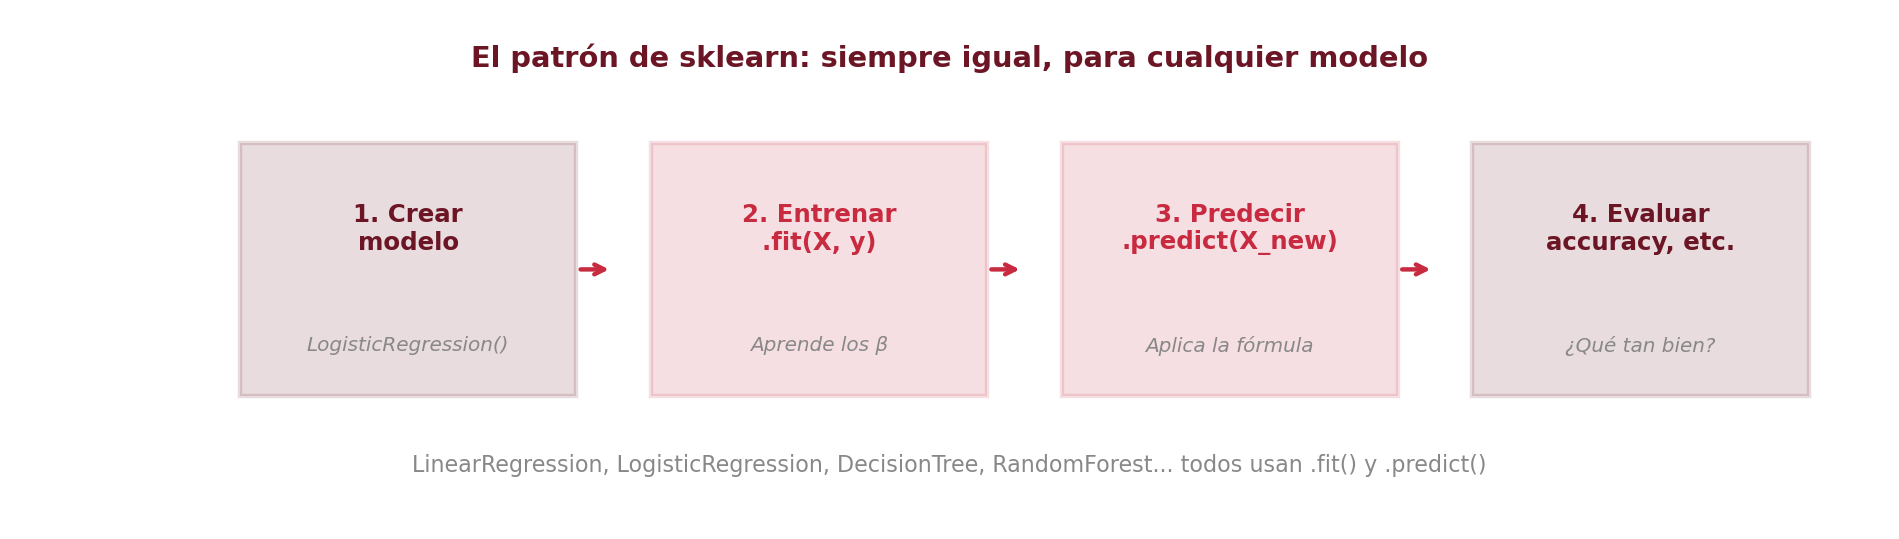
\includegraphics[width=0.92\textwidth]{img_flujo_sklearn.png}
  \end{center}

  \vspace{2pt}
  {\scriptsize\color{textMuted}
  \begin{itemize}\setlength{\itemsep}{2pt}
    \item[{\color{arcaRed}\scriptsize\faArrowRight}]
      \textbf{Crear}: \texttt{modelo = LinearRegression()} (o
      \texttt{LogisticRegression()}, o \texttt{DecisionTree()}\ldots).
    \item[{\color{arcaRed}\scriptsize\faArrowRight}]
      \textbf{Fit}: \texttt{modelo.fit(X\_train, y\_train)} ---
      el modelo ``aprende'' los $\beta$ a partir de los datos.
    \item[{\color{arcaRed}\scriptsize\faArrowRight}]
      \textbf{Predict}: \texttt{modelo.predict(X\_test)} ---
      aplica la fórmula aprendida a datos nuevos.
    \item[{\color{arcaRed}\scriptsize\faArrowRight}]
      \textbf{Evaluar}: comparar predicciones con la realidad (métricas).
  \end{itemize}
  }
\end{frame}

% =============================================================================
%  BLOQUE B: ¿Y SI EL TARGET ES SÍ/NO?
% =============================================================================
\sectionframe{¿Y Si el Target Es Sí/No?}{De predecir números a predecir categorías}

\begin{frame}[shrink=8]{Dos Tareas Fundamentales en Machine Learning}
  \vspace{-4pt}
  {\footnotesize\color{arcaDark}\bfseries
    En ML supervisado, todo problema cae en una de estas dos categorías.
    La diferencia es el \textbf{tipo de target}.}

  \vspace{6pt}
  \begin{columns}[T]
    \begin{column}{0.48\textwidth}
      {\footnotesize\bfseries\color{codeBlue}\faChartLine\hspace{4pt}
        Regresión:}
      \vspace{4pt}

      {\scriptsize
      El target es un \textbf{número continuo}.

      \vspace{4pt}
      \begin{itemize}\setlength{\itemsep}{4pt}
        \item ¿Cuánto \textbf{costará} el seguro? (\$)
        \item ¿Cuántas \textbf{unidades} vamos a vender?
        \item ¿Cuál será la \textbf{temperatura} mañana?
        \item ¿Cuánto \textbf{tiempo} tardará la entrega?
        \item ¿Cuál será el \textbf{precio} del producto?
      \end{itemize}
      }

      \vspace{4pt}
      {\scriptsize\color{codeBlue}\bfseries
        Métricas: MAE, RMSE, R\textsuperscript{2}}
    \end{column}

    \begin{column}{0.48\textwidth}
      {\footnotesize\bfseries\color{arcaRed}\faCheckCircle\hspace{4pt}
        Clasificación:}
      \vspace{4pt}

      {\scriptsize
      El target es una \textbf{categoría} (sí/no, A/B/C).

      \vspace{4pt}
      \begin{itemize}\setlength{\itemsep}{4pt}
        \item ¿El cliente \textbf{aceptará} la campaña? (sí/no)
        \item ¿La máquina va a \textbf{fallar}? (sí/no)
        \item ¿El correo es \textbf{spam}? (sí/no)
        \item ¿Qué \textbf{tipo} de producto es? (A/B/C)
        \item ¿El cliente hará \textbf{churn}? (sí/no)
      \end{itemize}
      }

      \vspace{4pt}
      {\scriptsize\color{arcaRed}\bfseries
        Métricas: accuracy, precision, recall}
    \end{column}
  \end{columns}

  \vspace{8pt}
  {\footnotesize\color{arcaDark}
    \faLightbulb\hspace{4pt}
    \textbf{La pregunta clave}: ¿tu target es un \textbf{número} o una
    \textbf{etiqueta}? Eso decide si es regresión o clasificación.
    Todo lo demás (flujo, código, sklearn) es igual.}
\end{frame}

\begin{frame}[shrink=5]{Un Nuevo Tipo de Problema}
  \vspace{-4pt}
  {\footnotesize\color{arcaDark}\bfseries
    En la clase 13 predijimos un \textbf{número} (\$). Pero muchas preguntas
    de negocio son de \textbf{sí o no}:}

  \vspace{8pt}
  {\footnotesize
  \begin{itemize}\setlength{\itemsep}{6pt}
    \item[{\color{arcaRed}\faArrowRight}]
      ¿Este cliente va a \textbf{aceptar} nuestra campaña de marketing?
    \item[{\color{arcaRed}\faArrowRight}]
      ¿Esta máquina va a \textbf{fallar} esta semana?
    \item[{\color{arcaRed}\faArrowRight}]
      ¿Este paciente tiene riesgo de \textbf{enfermedad} cardíaca?
    \item[{\color{arcaRed}\faArrowRight}]
      ¿Este empleado va a \textbf{renunciar}?
  \end{itemize}
  }

  \vspace{8pt}
  {\footnotesize\color{arcaDark}
    \faLightbulb\hspace{4pt}
    Cuando el target es \textbf{0/1} (no/sí), el problema se llama
    \textbf{clasificación binaria}.}
\end{frame}

\begin{frame}[shrink=5]{Nuevo Dataset: Bank Marketing}
  \vspace{-4pt}
  {\footnotesize\color{arcaDark}\bfseries
    Un banco llama a clientes para ofrecerles un depósito a plazo.
    ¿Aceptan o no?}

  \vspace{6pt}
  \begin{columns}[T]
    \begin{column}{0.48\textwidth}
      {\footnotesize\bfseries\color{arcaDark} Características:}
      \vspace{4pt}

      {\scriptsize
      \begin{itemize}\setlength{\itemsep}{3pt}
        \item[{\color{codeGreen}\faCheckCircle}]
          \textbf{45\,211} clientes, \textbf{23} columnas.
        \item[{\color{codeGreen}\faCheckCircle}]
          Sin valores faltantes.
        \item[{\color{codeGreen}\faCheckCircle}]
          Mezcla numérico + categórico.
        \item[{\color{codeGreen}\faCheckCircle}]
          Target: \texttt{response} (0 = no, 1 = sí).
      \end{itemize}
      }
    \end{column}

    \begin{column}{0.48\textwidth}
      {\footnotesize\bfseries\color{arcaDark} Variables clave:}
      \vspace{4pt}

      {\scriptsize
      \begin{itemize}\setlength{\itemsep}{3pt}
        \item \texttt{age} --- edad del cliente
        \item \texttt{job} --- tipo de trabajo
        \item \texttt{balance} --- saldo bancario
        \item \texttt{duration} --- duración de la llamada
        \item \texttt{campaign} --- llamadas en esta campaña
        \item \texttt{poutcome} --- resultado de campañas previas
      \end{itemize}
      }
    \end{column}
  \end{columns}

  \vspace{6pt}
  {\footnotesize\color{arcaDark}
    \faLightbulb\hspace{4pt}
    \textbf{Pregunta de negocio}: ¿a qué clientes debemos llamar para
    \textbf{no desperdiciar} tiempo ni presupuesto de marketing?}
\end{frame}

\begin{frame}[shrink=5]{Pregunta Provocadora}
  \vspace{-4pt}
  {\footnotesize\color{arcaDark}\bfseries
    Ya sabemos usar \texttt{LinearRegression}. El target es 0/1.
    ¿Podemos usar regresión lineal para predecir esto?}

  \vspace{10pt}
  \begin{center}
    {\Large\color{arcaRed}\bfseries
      Intentémoslo.}
  \end{center}

  \vspace{10pt}
  {\footnotesize\color{arcaDark}
    Vamos a hacer exactamente lo de la clase pasada:
    \texttt{train\_test\_split}, \texttt{get\_dummies},
    \texttt{LinearRegression().fit()}, \texttt{.predict()}
    --- y ver qué pasa.}
\end{frame}

\begin{frame}[fragile,shrink=35]{LinearRegression en Target Binario}
  \vspace{-6pt}
  {\footnotesize\color{arcaDark}\bfseries
    Mismo flujo de la clase 13. Mismo código. Target distinto.}

  \vspace{4pt}
  \begin{pyblock}
modelo_lineal = LinearRegression()
modelo_lineal.fit(X_train, y_train)

# Veamos que predice para 5 clientes del test
predicciones = modelo_lineal.predict(X_test[:5])
print("Predicciones:", predicciones.round(3))
  \end{pyblock}

  \vspace{4pt}
  \begin{outputblock}
Predicciones: [-0.017  0.025  0.196  0.205  0.060]
  \end{outputblock}

  \vspace{4pt}
  {\scriptsize\color{textMuted}
  \begin{itemize}\setlength{\itemsep}{3pt}
    \item[{\color{codeOrange}\scriptsize\faExclamationTriangle}]
      Predice $-0.017$. ¿Qué significa ``el cliente acepta $-1.7\%$''?
    \item[{\color{codeOrange}\scriptsize\faExclamationTriangle}]
      En otros casos predice $1.46$. ¿``Acepta 146\%''?
    \item[{\color{arcaRed}\scriptsize\faArrowRight}]
      \textbf{Los valores están fuera de [0, 1].} No son probabilidades
      válidas.
  \end{itemize}
  }
\end{frame}

\begin{frame}[shrink=5]{Pero Espera: ¿Y Si Ponemos un Umbral?}
  \vspace{-4pt}
  {\footnotesize\color{arcaDark}\bfseries
    Idea intuitiva: si la predicción es $>$ 0.5, decimos ``sí''.
    Si es $\leq$ 0.5, decimos ``no''.}

  \vspace{8pt}
  \begin{center}
    \begin{tcolorbox}[colback=arcaGray, colframe=arcaRed, boxrule=1pt,
                      arc=4pt, width=0.7\textwidth]
    \centering
    \footnotesize
    \texttt{y\_pred = (modelo.predict(X) > 0.5).astype(int)}
    \end{tcolorbox}
  \end{center}

  \vspace{6pt}
  {\footnotesize
  \begin{itemize}\setlength{\itemsep}{5pt}
    \item[{\color{arcaRed}\faArrowRight}]
      Predicción $= 0.7$ $\to$ \textbf{1} (sí acepta).
    \item[{\color{arcaRed}\faArrowRight}]
      Predicción $= 0.2$ $\to$ \textbf{0} (no acepta).
    \item[{\color{arcaRed}\faArrowRight}]
      Predicción $= -0.3$ $\to$ \textbf{0} (no acepta).
    \item[{\color{arcaRed}\faArrowRight}]
      Predicción $= 1.4$ $\to$ \textbf{1} (sí acepta).
  \end{itemize}
  }

  \vspace{6pt}
  {\footnotesize\color{arcaDark}
    \faLightbulb\hspace{4pt}
    \textbf{Funciona.} Pero ahora necesitamos \textbf{nuevas métricas}:
    ya no tiene sentido calcular MAE ni RMSE sobre predicciones 0/1.}
\end{frame}

% ── MÉTRICAS DE CLASIFICACIÓN ───────────────────────────────────────────────
\begin{frame}[shrink=5]{Nuevas Métricas: Accuracy}
  \vspace{-4pt}
  {\footnotesize\color{arcaDark}\bfseries
    La más simple de todas: ¿qué porcentaje acerté?}

  \vspace{6pt}
  \begin{center}
    \begin{tcolorbox}[colback=arcaGray, colframe=arcaRed, boxrule=1pt,
                      arc=4pt, width=0.55\textwidth]
    \centering
    \large
    $\text{Accuracy} = \dfrac{\text{predicciones correctas}}{\text{total}}$
    \end{tcolorbox}
  \end{center}

  \vspace{6pt}
  {\footnotesize
  \begin{itemize}\setlength{\itemsep}{5pt}
    \item[{\color{arcaRed}\faArrowRight}]
      Nuestro modelo lineal con umbral 0.5: \textbf{89.5\,\% accuracy}.
    \item[{\color{arcaRed}\faArrowRight}]
      Suena bien. \textbf{Pero cuidado\ldots}
    \item[{\color{codeOrange}\faExclamationTriangle}]
      Solo el 11.7\,\% de los clientes aceptan la campaña. Un modelo que
      \textbf{siempre diga ``no''} tendría 88.3\,\% de accuracy.
    \item[{\color{arcaRed}\faArrowRight}]
      \textbf{Accuracy sola no basta} cuando las clases están desbalanceadas.
  \end{itemize}
  }
\end{frame}

\begin{frame}[shrink=8]{Matriz de Confusión}
  \vspace{-4pt}
  {\footnotesize\color{arcaDark}\bfseries
    Para entender \textbf{en qué se equivoca} el modelo, necesitamos
    más detalle que un solo número.}

  \vspace{6pt}
  \begin{center}
  {\scriptsize
  \begin{tabular}{@{}l|cc@{}}
    & \textbf{Predicho: NO} & \textbf{Predicho: SÍ} \\
    \midrule
    \textbf{Real: NO} &
      {\color{codeGreen}\bfseries VN} (verdadero negativo) &
      {\color{codeOrange}\bfseries FP} (falso positivo) \\
    & Acerté: no acepta & Llamé innecesariamente \\
    \midrule
    \textbf{Real: SÍ} &
      {\color{arcaRed}\bfseries FN} (falso negativo) &
      {\color{codeGreen}\bfseries VP} (verdadero positivo) \\
    & No lo llamé y hubiera aceptado & Acerté: sí acepta \\
  \end{tabular}
  }
  \end{center}

  \vspace{6pt}
  {\footnotesize
  \begin{itemize}\setlength{\itemsep}{5pt}
    \item[{\color{arcaRed}\faArrowRight}]
      \textbf{¿Qué es peor?} Depende del negocio:
    \item[{\color{codeOrange}\scriptsize\faArrowRight}]
      \textbf{FP} (llamar a alguien que no acepta): pierdes \textbf{tiempo} del call center.
    \item[{\color{arcaRed}\scriptsize\faArrowRight}]
      \textbf{FN} (no llamar a alguien que hubiera aceptado): pierdes un \textbf{cliente}.
    \item[{\color{arcaRed}\scriptsize\faArrowRight}]
      Si perder un cliente cuesta más que una llamada, los \textbf{FN
      son más graves} que los FP.
  \end{itemize}
  }
\end{frame}

\begin{frame}[shrink=5]{Precision y Recall}
  \vspace{-4pt}
  {\footnotesize\color{arcaDark}\bfseries
    Dos formas de medir el rendimiento \textbf{enfocadas en la clase positiva}
    (los que sí aceptan).}

  \vspace{6pt}
  \begin{columns}[T]
    \begin{column}{0.48\textwidth}
      \begin{center}
        \begin{tcolorbox}[colback=arcaGray, colframe=arcaRed, boxrule=0.8pt,
                          arc=3pt, width=\textwidth]
        \centering
        \footnotesize
        $\text{Precision} = \dfrac{VP}{VP + FP}$
        \end{tcolorbox}
      \end{center}
      \vspace{4pt}
      {\scriptsize
      ``De los que dije SÍ, ¿cuántos \textbf{realmente} eran SÍ?''

      \vspace{4pt}
      Alta precision $=$ cuando digo ``sí'', casi siempre
      \textbf{acierto}. Pocas llamadas en vano.
      }
    \end{column}

    \begin{column}{0.48\textwidth}
      \begin{center}
        \begin{tcolorbox}[colback=arcaGray, colframe=arcaRed, boxrule=0.8pt,
                          arc=3pt, width=\textwidth]
        \centering
        \footnotesize
        $\text{Recall} = \dfrac{VP}{VP + FN}$
        \end{tcolorbox}
      \end{center}
      \vspace{4pt}
      {\scriptsize
      ``De los que \textbf{realmente} eran SÍ, ¿a cuántos los
      \textbf{detecté}?''

      \vspace{4pt}
      Alto recall $=$ \textbf{no me pierdo} clientes potenciales.
      Pero quizás llamo a muchos que no aceptan.
      }
    \end{column}
  \end{columns}

  \vspace{8pt}
  {\footnotesize\color{arcaDark}
    \faLightbulb\hspace{4pt}
    \textbf{Hay tensión} entre ambas: subir precision suele bajar recall
    y viceversa. La decisión depende del \textbf{costo de cada error}
    para el negocio.}
\end{frame}

\begin{frame}[shrink=5]{Nuestro Modelo Lineal con Umbral: Los Números}
  \vspace{-4pt}
  \begin{columns}[T]
    \begin{column}{0.48\textwidth}
      \begin{center}
        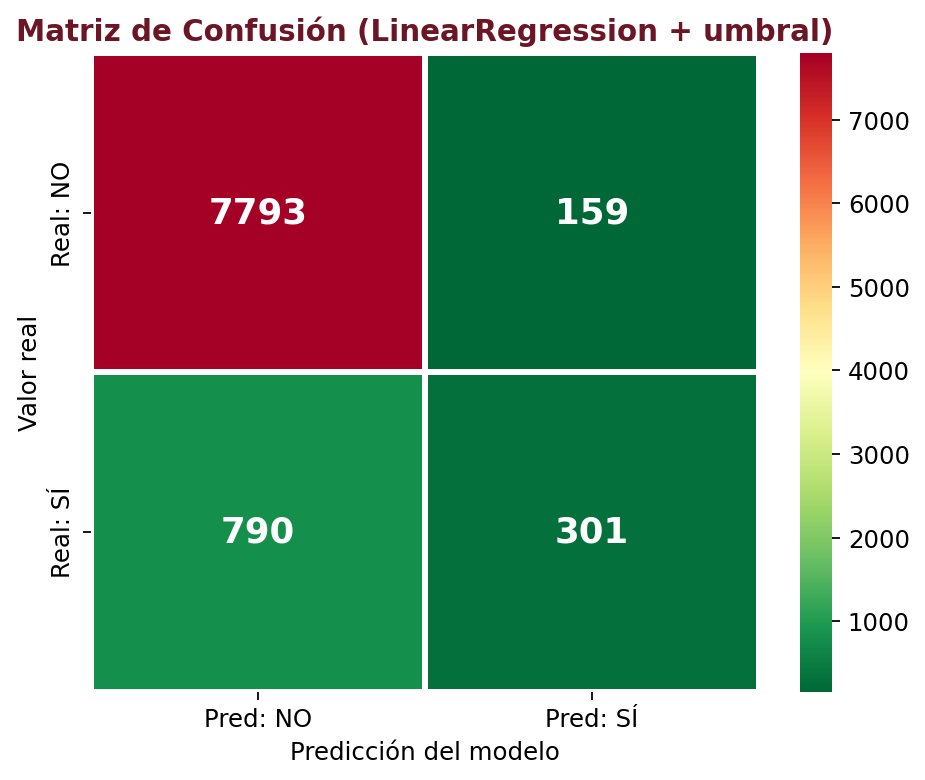
\includegraphics[width=\textwidth]{img_confusion_matrix.png}
      \end{center}
    \end{column}

    \begin{column}{0.48\textwidth}
      {\footnotesize\bfseries\color{arcaDark} Métricas:}
      \vspace{4pt}

      {\scriptsize
      \begin{tabular}{@{}lr@{}}
        \toprule
        \textbf{Métrica} & \textbf{Valor} \\
        \midrule
        Accuracy & 89.5\,\% \\
        Precision & 65.4\,\% \\
        Recall & 27.6\,\% \\
        \bottomrule
      \end{tabular}
      }

      \vspace{8pt}
      {\scriptsize\color{arcaDark}
        \faExclamationTriangle\hspace{4pt}
        \textbf{Recall = 27.6\,\%}: de los 1\,091
        clientes que habrían aceptado, el modelo
        solo detectó 301. Se le escaparon
        \textbf{790 clientes potenciales}.}
    \end{column}
  \end{columns}
\end{frame}

\begin{frame}[shrink=5]{El Problema de Fondo}
  \vspace{-4pt}
  {\footnotesize\color{arcaDark}\bfseries
    La regresión lineal ``funciona'' para clasificar, pero tiene dos
    problemas fundamentales:}

  \vspace{8pt}
  {\footnotesize
  \begin{itemize}\setlength{\itemsep}{8pt}
    \item[{\color{arcaRed}\faTimesCircle}]
      \textbf{Las predicciones no son probabilidades}: un valor de $-0.017$
      o $1.46$ no se puede interpretar como ``probabilidad de aceptar''.
      No podemos decir ``este cliente tiene 73\,\% de chance de decir sí''.
    \item[{\color{arcaRed}\faTimesCircle}]
      \textbf{No fue diseñada para esto}: OLS minimiza la suma de
      cuadrados, no la probabilidad de acertar la clase. Es como usar un
      destornillador para clavar un clavo --- se puede, pero hay
      herramientas mejores.
  \end{itemize}
  }

  \vspace{8pt}
  {\footnotesize\color{arcaDark}
    \faLightbulb\hspace{4pt}
    Necesitamos un modelo que: (1) prediga valores entre 0 y 1 siempre,
    y (2) esté optimizado para clasificar. Eso es la \textbf{regresión logística}.}
\end{frame}

% =============================================================================
%  BLOQUE C: REGRESIÓN LOGÍSTICA
% =============================================================================
\sectionframe{Regresión Logística}{La sigmoide y tu primer clasificador}

\begin{frame}{El Problema Visual: Lineal vs Logística}
  \vspace{-4pt}
  {\footnotesize\color{arcaDark}\bfseries
    La regresión lineal puede salirse de [0, 1]. La logística no.}

  \vspace{4pt}
  \begin{center}
    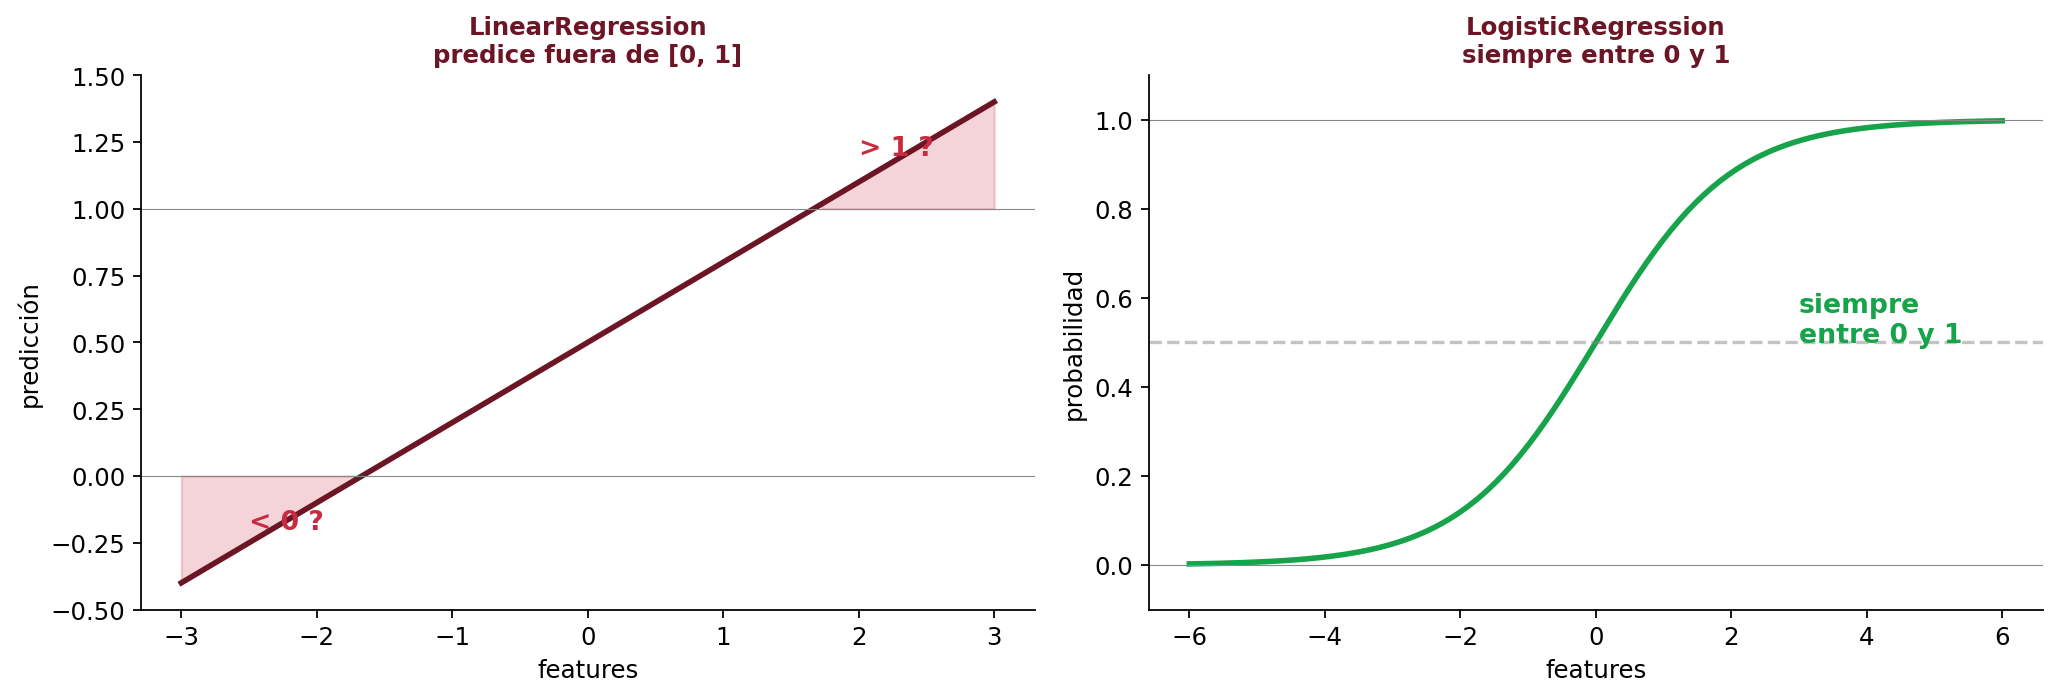
\includegraphics[width=0.92\textwidth]{img_lineal_vs_sigmoide.png}
  \end{center}

  \vspace{-2pt}
  {\scriptsize\color{textMuted}
  \begin{itemize}\setlength{\itemsep}{2pt}
    \item[{\color{arcaRed}\scriptsize\faArrowRight}]
      \textbf{Izquierda}: la regresión lineal puede predecir valores
      negativos o mayores que 1 (zonas rojas).
    \item[{\color{codeGreen}\scriptsize\faArrowRight}]
      \textbf{Derecha}: la sigmoide ``aplasta'' el resultado al rango
      [0, 1]. \textbf{Siempre} es una probabilidad válida.
  \end{itemize}
  }
\end{frame}

\begin{frame}{La Función Sigmoide: De Número a Probabilidad}
  \vspace{-4pt}
  {\footnotesize\color{arcaDark}\bfseries
    La regresión logística aplica esta función al resultado de la
    combinación lineal.}

  \vspace{2pt}
  \begin{center}
    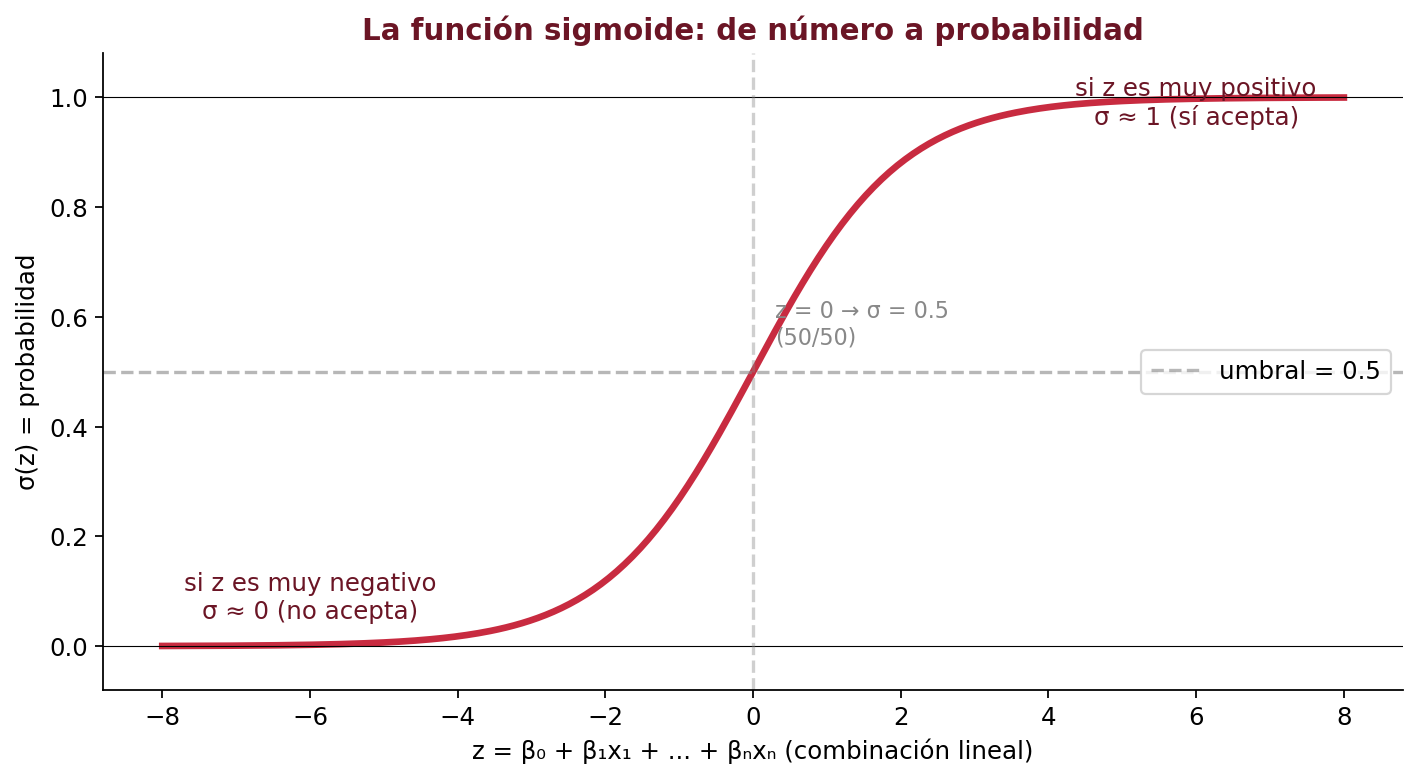
\includegraphics[width=0.52\textwidth]{img_sigmoide.png}
  \end{center}

  \vspace{2pt}
  {\scriptsize\color{textMuted}
  \begin{itemize}\setlength{\itemsep}{3pt}
    \item[{\color{arcaRed}\scriptsize\faArrowRight}]
      Entrada: $z = \beta_0 + \beta_1 x_1 + \ldots + \beta_n x_n$
      (la misma combinación lineal de siempre).
    \item[{\color{arcaRed}\scriptsize\faArrowRight}]
      Salida: $\sigma(z) = 1 / (1 + e^{-z})$ --- siempre entre 0 y 1.
    \item[{\color{arcaRed}\scriptsize\faArrowRight}]
      Si $\sigma > 0.5$: predecimos ``sí''. Si $\sigma \leq 0.5$:
      predecimos ``no''.
  \end{itemize}
  }
\end{frame}

\begin{frame}[fragile,shrink=35]{LogisticRegression: Una Línea de Diferencia}
  \vspace{-6pt}
  {\footnotesize\color{arcaDark}\bfseries
    Mismo flujo. Misma API. Una sola línea cambia.}

  \vspace{4pt}
  \begin{pyblock}
from sklearn.linear_model import LogisticRegression

modelo_log = LogisticRegression(max_iter=1000)
modelo_log.fit(X_train_s, y_train)

y_pred_log = modelo_log.predict(X_test_s)
print(f"Accuracy: {accuracy_score(y_test, y_pred_log):.4f}")
  \end{pyblock}

  \vspace{4pt}
  \begin{outputblock}
Accuracy: 0.8979
  \end{outputblock}

  \vspace{4pt}
  {\scriptsize\color{textMuted}
  \begin{itemize}\setlength{\itemsep}{3pt}
    \item[{\color{codeGreen}\scriptsize\faCheckCircle}]
      \textbf{89.8\,\%} (vs 89.5\,\% de la lineal). Ligeramente mejor.
    \item[{\color{arcaRed}\scriptsize\faArrowRight}]
      Pero la verdadera diferencia no está en accuracy\ldots
  \end{itemize}
  }
\end{frame}

\begin{frame}[fragile,shrink=35]{Lo Que Ganas: \texttt{predict\_proba()}}
  \vspace{-6pt}
  {\footnotesize\color{arcaDark}\bfseries
    La logística no solo dice ``sí o no''. Da la \textbf{probabilidad}.}

  \vspace{4pt}
  \begin{pyblock}
probas = modelo_log.predict_proba(X_test_s[:5])
print("     P(no)   P(si)")
for i, p in enumerate(probas):
    print(f"  Cliente {i}: {p[0]:.3f}    {p[1]:.3f}")
  \end{pyblock}

  \vspace{4pt}
  \begin{outputblock}
     P(no)   P(si)
  Cliente 0: 0.988    0.012
  Cliente 1: 0.976    0.024
  Cliente 2: 0.855    0.145
  Cliente 3: 0.772    0.228
  Cliente 4: 0.951    0.049
  \end{outputblock}

  \vspace{4pt}
  {\scriptsize\color{textMuted}
  \begin{itemize}\setlength{\itemsep}{3pt}
    \item[{\color{arcaRed}\scriptsize\faArrowRight}]
      Ahora \textbf{sí} puedes decir: ``este cliente tiene un 22.8\,\% de
      probabilidad de aceptar''.
    \item[{\color{arcaRed}\scriptsize\faArrowRight}]
      Eso es \textbf{imposible} con \texttt{LinearRegression}.
  \end{itemize}
  }
\end{frame}

\begin{frame}[shrink=8]{Comparación: Lineal vs Logística}
  \vspace{-4pt}
  {\footnotesize\color{arcaDark}\bfseries
    Los dos modelos lado a lado.}

  \vspace{6pt}
  {\scriptsize
  \begin{tabular}{@{}lcc@{}}
    \toprule
    & \textbf{LinearRegression + umbral} & \textbf{LogisticRegression} \\
    \midrule
    Accuracy & 89.5\,\% & \textbf{89.8\,\%} \\
    Precision & 65.4\,\% & \textbf{65.3\,\%} \\
    Recall & 27.6\,\% & \textbf{32.8\,\%} \\
    Probabilidades reales & \color{arcaRed}\faTimesCircle\color{textDark}\hspace{2pt} No &
      \color{codeGreen}\faCheckCircle\color{textDark}\hspace{2pt} Sí \\
    Predicciones fuera de [0, 1] & \color{arcaRed}\faTimesCircle\color{textDark}\hspace{2pt} Sí &
      \color{codeGreen}\faCheckCircle\color{textDark}\hspace{2pt} No \\
    Diseñada para clasificar & \color{arcaRed}\faTimesCircle\color{textDark}\hspace{2pt} No &
      \color{codeGreen}\faCheckCircle\color{textDark}\hspace{2pt} Sí \\
    \bottomrule
  \end{tabular}
  }

  \vspace{6pt}
  {\footnotesize
  \begin{itemize}\setlength{\itemsep}{4pt}
    \item[{\color{codeGreen}\faCheckCircle}]
      \textbf{Recall subió de 27.6 a 32.8\,\%}: la logística detecta
      \textbf{57 clientes más} que aceptarían (358 vs 301).
    \item[{\color{codeGreen}\faCheckCircle}]
      \texttt{predict\_proba()} permite ajustar el umbral según el
      costo de cada error para el negocio.
  \end{itemize}
  }
\end{frame}

\begin{frame}[shrink=5]{El Flujo Completo --- Otra Vez}
  \vspace{-4pt}
  {\footnotesize\color{arcaDark}\bfseries
    ¿Recuerdan el flujo de la clase 13? No cambió nada.}

  \vspace{8pt}
  \begin{center}
  \begin{tikzpicture}[
    node distance=0.4cm,
    box/.style={rectangle, rounded corners=4pt, draw=arcaRed, fill=arcaRed!8,
                minimum width=2.6cm, minimum height=0.9cm,
                font=\footnotesize\bfseries\color{arcaDark}, align=center},
    arr/.style={->, >=Stealth, thick, arcaRed},
  ]
    \node[box] (b1) {1. Split\\\scriptsize train/test};
    \node[box, right=of b1] (b2) {2. Encode\\\scriptsize categóricas};
    \node[box, right=of b2] (b3) {3. Scale\\\scriptsize estandarizar};
    \node[box, right=of b3] (b4) {4. Fit\\\scriptsize entrenar};
    \node[box, right=of b4] (b5) {5. Evaluate\\\scriptsize en test};

    \draw[arr] (b1) -- (b2);
    \draw[arr] (b2) -- (b3);
    \draw[arr] (b3) -- (b4);
    \draw[arr] (b4) -- (b5);
  \end{tikzpicture}
  \end{center}

  \vspace{8pt}
  {\footnotesize
  \begin{itemize}\setlength{\itemsep}{4pt}
    \item[{\color{arcaRed}\faArrowRight}]
      Clase 13: usaron \texttt{LinearRegression()} para predecir un \textbf{número}.
    \item[{\color{arcaRed}\faArrowRight}]
      Hoy: usaron \texttt{LogisticRegression()} para predecir un \textbf{sí/no}.
    \item[{\color{arcaRed}\faArrowRight}]
      \textbf{El flujo es idéntico.} Solo cambiaron el modelo y las métricas.
  \end{itemize}
  }
\end{frame}

% =============================================================================
%  BLOQUE D: CIERRE DEL MÓDULO 2
% =============================================================================
\sectionframe{Cierre del Módulo 2}{El mapa completo}

\begin{frame}[shrink=5]{Los Dos Tipos de Problemas Supervisados}
  \vspace{-4pt}
  {\footnotesize\color{arcaDark}\bfseries
    Después de 7 clases de estadística, tienen los dos pilares
    del machine learning supervisado.}

  \vspace{8pt}
  \begin{columns}[T]
    \begin{column}{0.48\textwidth}
      {\footnotesize\bfseries\color{codeBlue}\faChartLine\hspace{4pt}
        Regresión:}
      \vspace{4pt}

      {\scriptsize
      \begin{itemize}\setlength{\itemsep}{4pt}
        \item Target: un \textbf{número} (\$, kg, litros\ldots)
        \item Modelo: \texttt{LinearRegression}
        \item Métricas: MAE, RMSE, R\textsuperscript{2}
        \item Ejemplo: predecir costo del seguro
      \end{itemize}
      }
    \end{column}

    \begin{column}{0.48\textwidth}
      {\footnotesize\bfseries\color{arcaRed}\faCheckCircle\hspace{4pt}
        Clasificación:}
      \vspace{4pt}

      {\scriptsize
      \begin{itemize}\setlength{\itemsep}{4pt}
        \item Target: una \textbf{categoría} (sí/no, A/B/C\ldots)
        \item Modelo: \texttt{LogisticRegression}
        \item Métricas: accuracy, precision, recall, confusión
        \item Ejemplo: predecir respuesta de campaña
      \end{itemize}
      }
    \end{column}
  \end{columns}

  \vspace{8pt}
  {\footnotesize\color{arcaDark}
    \faLightbulb\hspace{4pt}
    En el \textbf{Módulo 4} van a aprender modelos más potentes (árboles,
    random forest, gradient boosting\ldots), pero todos se dividen en
    estos mismos dos tipos. Y todos usan el mismo flujo
    \texttt{split} $\to$ \texttt{fit} $\to$ \texttt{predict} $\to$
    \texttt{evaluar}.}
\end{frame}

\begin{frame}{Lo que Aprendimos en el Módulo 2}
  \vspace{-4pt}
  \begin{columns}[T]
    \begin{column}{0.48\textwidth}
      {\footnotesize
      \begin{itemize}\setlength{\itemsep}{4pt}
        \item[{\color{codeGreen}\faCheckCircle}]
          EDA: conocer tus datos.
        \item[{\color{codeGreen}\faCheckCircle}]
          Distribuciones, outliers, Normal.
        \item[{\color{codeGreen}\faCheckCircle}]
          Correlación: Pearson, Spearman.
        \item[{\color{codeGreen}\faCheckCircle}]
          Categóricas y encoding.
      \end{itemize}
      }
    \end{column}

    \begin{column}{0.48\textwidth}
      {\footnotesize
      \begin{itemize}\setlength{\itemsep}{4pt}
        \item[{\color{codeGreen}\faCheckCircle}]
          Regresión lineal, métricas, p-values.
        \item[{\color{codeGreen}\faCheckCircle}]
          Train/test split, overfitting.
        \item[{\color{codeGreen}\faCheckCircle}]
          Estandarización (z-score reaparece).
        \item[{\color{codeGreen}\faCheckCircle}]
          Regresión logística y clasificación.
      \end{itemize}
      }
    \end{column}
  \end{columns}

  \vspace{6pt}
  {\small\color{arcaDark}\bfseries Próximo módulo (lunes 13):}
  \vspace{2pt}
  {\footnotesize
  \begin{itemize}\setlength{\itemsep}{2pt}
    \item[{\color{arcaRed}\faArrowRight}]
      \textbf{Módulo 3: Análisis y Visualización de Datos.}
    \item[{\color{arcaRed}\faArrowRight}]
      Ya saben modelar. Ahora van a aprender a \textbf{contar la historia}
      de los datos con gráficos.
  \end{itemize}
  }
\end{frame}

% ── QR ENCUESTA ──────────────────────────────────────────────────────────────
{
\setbeamertemplate{headline}{}
\setbeamertemplate{footline}{}
\begin{frame}[plain, noframenumbering]
  \begin{tikzpicture}[remember picture, overlay]
    \fill[arcaDark] (current page.south west) rectangle (current page.north east);
  \end{tikzpicture}
  \vspace{1cm}
  \begin{center}
    {\Huge\bfseries\color{white} ¿Cómo estuvo la clase?\par}
    \vspace{0.6cm}
    
\includegraphics[width=4cm]{qr_encuesta.jpg}
    \vspace{0.4cm}

    {\large\color{white!80} Escanea el QR para dejarnos tu opinión.\par}
  \end{center}
\end{frame}
}

\end{document}
